\documentclass[10pt]{extarticle}\usepackage[]{graphicx}\usepackage[]{color}
%% maxwidth is the original width if it is less than linewidth
%% otherwise use linewidth (to make sure the graphics do not exceed the margin)
\makeatletter
\def\maxwidth{ %
  \ifdim\Gin@nat@width>\linewidth
    \linewidth
  \else
    \Gin@nat@width
  \fi
}
\makeatother

\definecolor{fgcolor}{rgb}{0.345, 0.345, 0.345}
\newcommand{\hlnum}[1]{\textcolor[rgb]{0.686,0.059,0.569}{#1}}%
\newcommand{\hlstr}[1]{\textcolor[rgb]{0.192,0.494,0.8}{#1}}%
\newcommand{\hlcom}[1]{\textcolor[rgb]{0.678,0.584,0.686}{\textit{#1}}}%
\newcommand{\hlopt}[1]{\textcolor[rgb]{0,0,0}{#1}}%
\newcommand{\hlstd}[1]{\textcolor[rgb]{0.345,0.345,0.345}{#1}}%
\newcommand{\hlkwa}[1]{\textcolor[rgb]{0.161,0.373,0.58}{\textbf{#1}}}%
\newcommand{\hlkwb}[1]{\textcolor[rgb]{0.69,0.353,0.396}{#1}}%
\newcommand{\hlkwc}[1]{\textcolor[rgb]{0.333,0.667,0.333}{#1}}%
\newcommand{\hlkwd}[1]{\textcolor[rgb]{0.737,0.353,0.396}{\textbf{#1}}}%
\let\hlipl\hlkwb

\usepackage{framed}
\makeatletter
\newenvironment{kframe}{%
 \def\at@end@of@kframe{}%
 \ifinner\ifhmode%
  \def\at@end@of@kframe{\end{minipage}}%
  \begin{minipage}{\columnwidth}%
 \fi\fi%
 \def\FrameCommand##1{\hskip\@totalleftmargin \hskip-\fboxsep
 \colorbox{shadecolor}{##1}\hskip-\fboxsep
     % There is no \\@totalrightmargin, so:
     \hskip-\linewidth \hskip-\@totalleftmargin \hskip\columnwidth}%
 \MakeFramed {\advance\hsize-\width
   \@totalleftmargin\z@ \linewidth\hsize
   \@setminipage}}%
 {\par\unskip\endMakeFramed%
 \at@end@of@kframe}
\makeatother

\definecolor{shadecolor}{rgb}{.97, .97, .97}
\definecolor{messagecolor}{rgb}{0, 0, 0}
\definecolor{warningcolor}{rgb}{1, 0, 1}
\definecolor{errorcolor}{rgb}{1, 0, 0}
\newenvironment{knitrout}{}{} % an empty environment to be redefined in TeX

\usepackage{alltt}

\usepackage{underscore}
\usepackage[utf8]{inputenc}
\usepackage{longtable}
\usepackage[margin=1in]{geometry}
\usepackage[spanish]{babel}
\usepackage{hyperref}
\usepackage{graphicx}
\usepackage{fancyvrb}
\usepackage{anysize}
\usepackage{subfig}
\usepackage{wrapfig}
\usepackage{fancyhdr}

\marginsize{2.5cm}{2.5cm}{3cm}{3cm}
%\SweaveOpts{echo=false}
\renewcommand{\baselinestretch}{1.3} % per canviar interlineado

% Referencies amb vermell

%----------------------------------------------------------------------------------------
%  TITLE PAGE
%----------------------------------------------------------------------------------------
\newcommand*{\titleGM}{\begingroup % Create the command for including the title page in the document
\hbox{ % Horizontal box
\hspace*{0.2\textwidth} % Whitespace to the left of the title page
\rule{1pt}{\textheight} % Vertical line
\hspace*{0.05\textwidth} % Whitespace between the vertical line and title page text
\parbox[b]{0.75\textwidth}{ % Paragraph box which restricts text to less than the width of the page

{\noindent\Huge\bfseries Ejercicio: \\ Contrastes de hipotesis \\ \\ EBB}\\[2\baselineskip] % Title

{\Large \textsc{Santi Pérez-Hoyos, \\ Miriam Mota, \\ Alex Sánchez }} % Author name

\vspace{0.4\textheight} % Whitespace between the title block and the publisher
%{\noindent Tutores: \\ \textsc{Alex S\'anchez \\ Juan Ram\'on Gonz\'alez}}\\[\baselineskip] % Publisher and logo
}}
\endgroup}



%----------------------------------------------------------------------------------------
%  BLANK DOCUMENT
%----------------------------------------------------------------------------------------
\IfFileExists{upquote.sty}{\usepackage{upquote}}{}
\begin{document}




% http://en.wikibooks.org/wiki/LaTeX/Page_Layout

\titleGM % This command includes the title page

\clearpage

\pagestyle{fancy} % Removes page numbers


%----------------------------------------------------------------------------------------
\section{Ejercicio}
%----------------------------------------------------------------------------------------
\textbf{Indica que tipo de análisis o que pruebas estadísticas utilizarías y si fuera necesario algún tipo de prueba adicional para llevar a cabo el análisis. Formula la hipótesis a contrastar de acuerdo con las hipótesis seleccionadas}
\begin{enumerate}
  \item [a.] \textbf{Se efectúa un estudio de seguimiento a 1018 sujetos atendidos en una clínica de obesidad. Se mide el Indice de Masa Corporal(IMC) y el perfil lipídico. Al cabo de 12 meses se evalúa de nuevo el IMC y el colesterol estando interesados en cuantificar la disminución de ambos parámetros}\\
  
  Disponemos de dos variables cuantitativas medidas en dos momentos distintos. Se quiere analizar si los valores pre y post sufren algun cambio, para ello debemos: en primer lugar evaluar la normalidad de las variables. En caso de que se ajusten a una distribución normal, miramos la homegeneidad de las variables y realizamos un test t de Student para muestras apareadas. En el caso de que no sigan una distribución normal, realizaremos el test no paramétrico de wilcoxon para muestras apareadas. 

  \item [b.] \textbf{Se analizan un grupo de variables inmunológica(leucocitos totales, linfocitos B, natural Killer, etc) en una muestra de 102 hombres y 147 mujeres mayores de 65 años. Se está interesado en ver la existencia de diferencias por sexo.}\\
  
  Disponemos de distintas variables cuantitativas (leucocitos,linfocitos, etc. ) y una variable cualitativa, sexo. Queremos ver si existen diferencias de las variables cuantitativas según el sexo, para ello debemos: en primer lugar evaluar la normalidad de las variables. En caso de que se ajusten a una distribución normal, miramos la homegeneidad de las variables y realizamos un test t de Student. En el caso de que no sigan una distribución normal, realizaremos el test no paramétrico U de Mann-Whitnney. 

  \item [c.] \textbf{La supervivencia de los pacientes con cardiopatía isquémica se asocia al valor de la fracción de eyección(FE). Se desea comparar los resultados obtenidos en 125 pacientes mediante la fracción de eyección isotópica en la asignación de sujetos a grupos de alto y bajo riesgo con la asignación obtenida a partir de la FE angiográfica. Plantea el análisis.}\\

Disponemos de dos variables cualitativas, queremos ver si existe relación entre el riesgo y la clasificacio según FE angiográfica, para ello debemos: en primer lugar realizamos una tabla de frecuencias, en el caso de obtener en alguna celda un valor inferior a 0.05 realizamos un test exacto de Fisher, en caso contrario un test Chi Cuadrado. 

\end{enumerate}


%----------------------------------------------------------------------------------------
\section{Ejercicio Práctico}
%----------------------------------------------------------------------------------------
\textbf{Este ejercicio consta de diversas partes en un intento de simular lo que se lleva a cabo en un estudio real. Se ha simplificado para hacerlo más practicable por lo que no hace falta que os agobiéis si algo no os cuadre del todo. De lo que se trata es que veamos como aplicar las distintas técnicas que hemos estudiado, de forma integral, en un problema de análisis de datos.}

\subsection{Los datos}
\textbf{La demora entre el comienzo de los síntomas y el ingreso hospitalario es un factor que determina la mortalidad del infarto agudo de miocardio (IAM). Se estudian 426 sujetos que acuden al servicio de urgencias de 5 hospitales por dolor torácico , recogiendo el tiempo entre los primeros síntomas y la llegada al hospital y una serie de variables sociodemográficas. Se está interesado en estimar el retraso prehospitalario y determinar las variables asociadas. Los datos los podéis encontrar en los ficheros de Stata demora.dta, de Excel demora.xls y de texto plano separado por comas demora.csv}

\begin{figure}[ht]
\centering
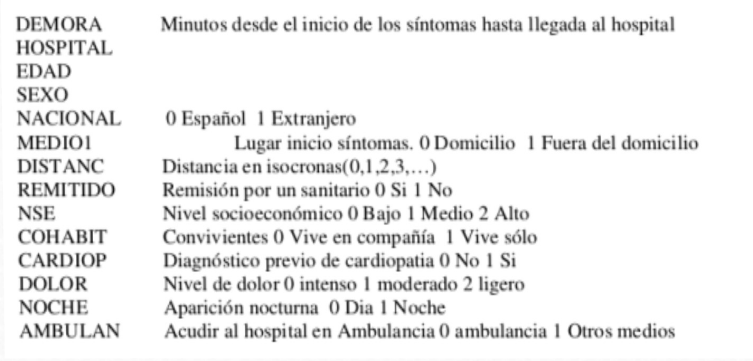
\includegraphics[width=0.851\textwidth, height=0.3\textheight]{Selection240.png}\\
\end{figure}

\begin{knitrout}
\definecolor{shadecolor}{rgb}{0.969, 0.969, 0.969}\color{fgcolor}\begin{kframe}
\begin{alltt}
\hlstd{dat} \hlkwb{<-} \hlkwd{read.csv}\hlstd{(}\hlstr{"demora.csv"}\hlstd{)}
\hlstd{dat}\hlopt{$}\hlstd{noche} \hlkwb{<-} \hlkwd{factor}\hlstd{(dat}\hlopt{$}\hlstd{noche,} \hlnum{0}\hlopt{:}\hlnum{1}\hlstd{,} \hlkwd{c}\hlstd{(}\hlstr{"Dia"}\hlstd{,} \hlstr{"Noche"}\hlstd{))}
\hlstd{dat}\hlopt{$}\hlstd{noche} \hlkwb{<-} \hlkwd{relevel}\hlstd{(dat}\hlopt{$}\hlstd{noche,}\hlkwc{ref} \hlstd{=} \hlstr{"Noche"}\hlstd{)}
\end{alltt}
\end{kframe}
\end{knitrout}




\newpage
\subsection{Los análisis}

\begin{enumerate}
  \item [a)] \textbf{Se está interesado en conocer la relación entre la demora y la aparición nocturna del síntoma.}
    \begin{itemize}
      \item \textbf{Comprueba la normalidad de la variable}\\
Realizamos gráficos y test de normalidad shapiro Wilks.
\begin{knitrout}
\definecolor{shadecolor}{rgb}{0.969, 0.969, 0.969}\color{fgcolor}\begin{kframe}
\begin{alltt}
\hlkwd{qqnorm}\hlstd{(dat}\hlopt{$}\hlstd{demora)}
\hlkwd{qqline}\hlstd{(dat}\hlopt{$}\hlstd{demora)}
\end{alltt}
\end{kframe}
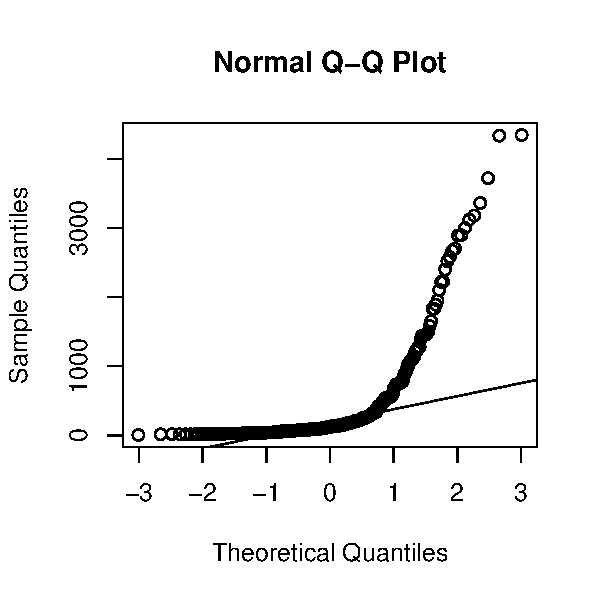
\includegraphics[width=\maxwidth]{figure/unnamed-chunk-2-1} 
\begin{kframe}\begin{alltt}
\hlkwd{shapiro.test}\hlstd{(dat}\hlopt{$}\hlstd{demora)}
\end{alltt}
\begin{verbatim}
## 
## 	Shapiro-Wilk normality test
## 
## data:  dat$demora
## W = 0.55371, p-value < 2.2e-16
\end{verbatim}
\end{kframe}
\end{knitrout}
      
Con un p-valor inferior a 0.05 concluimos que los datos no se ajustan a una distribución normal. 
      
      \item \textbf{Indica el procedimiento de análisis.}\\
      En primer lugar, debemos realizar un análisis gráfico. \\
      
      Dado que los datos no se ajustan a una distribución normal, las pruebas que usemos deberan ser no paramétricas. 
      
      
      \item \textbf{Aunque no sea el método más adecuado realiza el contraste paramétrico para contrastar la existencia de relación. Interpreta los resultados}
      
\begin{knitrout}
\definecolor{shadecolor}{rgb}{0.969, 0.969, 0.969}\color{fgcolor}\begin{kframe}
\begin{alltt}
\hlkwd{t.test}\hlstd{(dat}\hlopt{$}\hlstd{demora} \hlopt{~} \hlstd{dat}\hlopt{$}\hlstd{noche)}
\end{alltt}
\begin{verbatim}
## 
## 	Welch Two Sample t-test
## 
## data:  dat$demora by dat$noche
## t = 4.7841, df = 104.89, p-value = 5.641e-06
## alternative hypothesis: true difference in means is not equal to 0
## 95 percent confidence interval:
##  313.873 758.213
## sample estimates:
## mean in group Noche   mean in group Dia 
##            780.3061            244.2632
\end{verbatim}
\end{kframe}
\end{knitrout}
  Con un p-valor inferior a 0.05 rechazamos la hipotesis nula de igualdad de medias. Concluimos que se aprecian diferencia entre los tiempos al acudir al hospital entre los paciente a los que les sucede en eventos de dia o de noche.\\
  
  A esta misma conlusión podemos llegar si observamos el intervalo de confianza, ya que, no incluye el 0. 
  
  
      
      
      \item \textbf{Aunque no sea el método más adecuado realiza el contraste no paramétrico para contrastar la existencia de relación. Interpreta los resultados}\\
      
\begin{knitrout}
\definecolor{shadecolor}{rgb}{0.969, 0.969, 0.969}\color{fgcolor}\begin{kframe}
\begin{alltt}
\hlkwd{wilcox.test}\hlstd{(dat}\hlopt{$}\hlstd{demora} \hlopt{~} \hlstd{dat}\hlopt{$}\hlstd{noche)}
\end{alltt}
\begin{verbatim}
## 
## 	Wilcoxon rank sum test with continuity correction
## 
## data:  dat$demora by dat$noche
## W = 18300, p-value = 4.49e-06
## alternative hypothesis: true location shift is not equal to 0
\end{verbatim}
\end{kframe}
\end{knitrout}
    
    Con un p-valor inferior a 0.05, rechazamos la hipotésis nula. Tenemos evidencias estadísticas en que hay diferencia en el tiempo de demora al hospital para los distintos grupos (dia-noche)  
    
    
      \item \textbf{Justifica cual es la mejor opción de las efectuadas anteriormente}\\
      De forma teórica (y basandonos en no normalidad) escogeriamos el test U de Mann-Withney. Usemos el test paramétrico o no paramétrico llegamos a la misma conclusión. 
    \end{itemize}

  \item [b)] \textbf{Se cree que a un 20\% de los pacientes les aparecen los síntomas por la noche. Comprueba dicha hipotesis. Que conclusión se obtiene?}
  
  Realizamos un test de proporciones para una muestra. Con un p-valor inferior a 0.05 rechazamos que al 20\% de los pacientes les aparezcan los síntomas por la noche. 
\begin{knitrout}
\definecolor{shadecolor}{rgb}{0.969, 0.969, 0.969}\color{fgcolor}\begin{kframe}
\begin{alltt}
\hlkwd{prop.test}\hlstd{(}\hlkwd{table}\hlstd{(dat}\hlopt{$}\hlstd{noche),}\hlkwc{p} \hlstd{=} \hlnum{.2}\hlstd{)}
\end{alltt}
\begin{verbatim}
## 
## 	1-sample proportions test with continuity correction
## 
## data:  table(dat$noche), null probability 0.2
## X-squared = 44.866, df = 1, p-value = 2.11e-11
## alternative hypothesis: true p is not equal to 0.2
## 95 percent confidence interval:
##  0.2868619 0.3782098
## sample estimates:
##         p 
## 0.3309859
\end{verbatim}
\end{kframe}
\end{knitrout}
  
  
  \item [c)] \textbf{Se esta interesado en estudiar la relación entre el nivel de dolor y la aparición nocturna de los sintomas. }
  \begin{itemize}
    \item \textbf{Indica el procedimiento de análisis.}
    Realizamos una tabla de frecuencias para ver como se distribuyen los datos y si en alguna de las celdas tenemos un valor inferior a 5, si es así realizamos un test exacto de Fisher, en caso contrario un test chi cuadrado para evaluar independencia entre variables.
    \item \textbf{Ejecuta dicho análisis e interpreta los resultados.}
\begin{knitrout}
\definecolor{shadecolor}{rgb}{0.969, 0.969, 0.969}\color{fgcolor}\begin{kframe}
\begin{alltt}
\hlstd{gmodels}\hlopt{::}\hlkwd{CrossTable}\hlstd{(dat}\hlopt{$}\hlstd{dolor, dat}\hlopt{$}\hlstd{noche,} \hlkwc{prop.c} \hlstd{= F,}\hlkwc{prop.r} \hlstd{= F,}\hlkwc{chisq} \hlstd{= F,}\hlkwc{prop.chisq} \hlstd{= F)}
\end{alltt}
\begin{verbatim}
## 
##  
##    Cell Contents
## |-------------------------|
## |                       N |
## |         N / Table Total |
## |-------------------------|
## 
##  
## Total Observations in Table:  426 
## 
##  
##              | dat$noche 
##    dat$dolor |     Noche |       Dia | Row Total | 
## -------------|-----------|-----------|-----------|
##            0 |        68 |       137 |       205 | 
##              |     0.160 |     0.322 |           | 
## -------------|-----------|-----------|-----------|
##            1 |        59 |       124 |       183 | 
##              |     0.138 |     0.291 |           | 
## -------------|-----------|-----------|-----------|
##            2 |        14 |        24 |        38 | 
##              |     0.033 |     0.056 |           | 
## -------------|-----------|-----------|-----------|
## Column Total |       141 |       285 |       426 | 
## -------------|-----------|-----------|-----------|
## 
## 
\end{verbatim}
\end{kframe}
\end{knitrout}
    Como ningun valor de la tabla es inferior a 5 realizamos un test chi-cuadrado. 
\begin{knitrout}
\definecolor{shadecolor}{rgb}{0.969, 0.969, 0.969}\color{fgcolor}\begin{kframe}
\begin{alltt}
\hlkwd{chisq.test}\hlstd{(}\hlkwd{table}\hlstd{(dat}\hlopt{$}\hlstd{dolor, dat}\hlopt{$}\hlstd{noche))}
\end{alltt}
\begin{verbatim}
## 
## 	Pearson's Chi-squared test
## 
## data:  table(dat$dolor, dat$noche)
## X-squared = 0.30183, df = 2, p-value = 0.8599
\end{verbatim}
\end{kframe}
\end{knitrout}
    Con los resultados del test, p.valor superior a 0.05, no podemos rechazar la hipotesis nula,consideramos que noche y dolor son independientes.
  \end{itemize}
    

\end{enumerate}


% \begin{figure}[ht]
% \centering
% \subfloat{\includegraphics[width=0.71\textwidth, height=0.3\textheight]{results/Selection229.png}}\\
% \subfloat{\includegraphics[width=0.71\textwidth, height=0.3\textheight]{results/Selection230.png}} % \newline 
% \caption{Ejercicio 1}
% \label {descr}
% \end{figure}
% \clearpage






\end{document}
